\setlength{\parindent}{2em}   % 2em first-line indent for all paragraphs
\setlength{\parskip}{0pt}     % remove extra spacing between paragraphs

\section{Technology Assignment}
\noindent \textbf{Assignment 1: Marker oxidation}

\noindent \textbf{As mentioned above, the waferstepper alignment markers are the first step of the process. For the waferstepper to see this markers with a laser, a step has to be formed in the silicon. A way of forming this step is by performing a double oxidation. Here you will calculate the step height made in the Si wafer during this process.}

\noindent \textbf{The oxidation rate of silicon is given by the following equation (Deal-Grove model):
\begin{align*}
    \frac{dx}{dt} = \frac{B}{2x + A}
\end{align*}
where $x$ = oxide thickness, $A$ and $B$ are constants.}

\vspace{0.5em}
\noindent \textbf{a) Show that the solution of this equation for $t$ with $x = x_0$ at $t = 0$ as initial condition is:
\[
t = \frac{(x^2 - x_0^2) + A(x - x_0)}{B}
\]}

From 
\begin{gather*}
    \frac{dx}{dt} = \frac{B}{2x + A},
\end{gather*}

Rewrite the derivative above as
\begin{gather*}
    (2x+A)dx = Bdt
\end{gather*}

Integrate the left side from $x_0$ to $x$ and the right side from $0$ to $t$ respectively
\begin{gather*}
    \int_{x_0}^{x} (2x + A)dx = \int_{0}^{t} Bdt \\
    (x^2 - x_0^2) + A(x - x_0) = Bt \\
\end{gather*}

Therefore,  the solution of this equation for t with $x = x_0$ at $t = 0$ as initial condition is
\begin{gather*}
    t = \frac{(x^2 - x_0^2) + A(x - x_0)}{B}
\end{gather*}

\vspace{0.5em}
\noindent \textbf{At 1100$^{\circ}$C the constants are: $B=0.553 \ \mu\mathrm{m}^2/\mathrm{hr}$ and $B/A=3.1695 \ \mu\mathrm{m}/\mathrm{hr}$.} \\[0.5ex]
\noindent \textbf{b) Calculate the oxide thickness after the first oxidation (time=38.5 min).}

\noindent \textbf{Now a window is etched in the $SiO_2$ to make the marker, as hsown in the figure below, after which another oxidation is performed.}
\begin{figure}
\end{figure}

From $B =0.553$, $\frac{B}{A} =3.1695$ and $A = \frac{B}{\frac{B}{A}} \approx 0.1745$ and $t = 38.5$ min $ \approx 0.6417$ hr and $x_0$ before the first oxidation is 0, 
\begin{gather*}
    t = \frac{x^2+Ax}{B} \\
    x^2 + Ax - Bt = 0 \\
    x^2+0.1745x-0.3548=0 \\
\end{gather*}

This equation gives two roots, which are $x \approx 0.5147$ and $x \approx -0.6893$ (discarded). Therefore, the first oxide thickness is $0.5147 \mu\mathrm{m}$



\vspace{0.5em}
\begin{figure}[H]
    \centering
    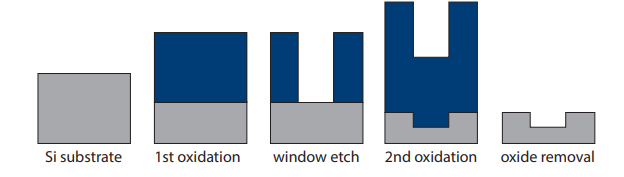
\includegraphics[width=0.7\linewidth]{Figures/tech_assignment_1_c.png}
    \label{fig:placeholder}
\end{figure}
\noindent \textbf{c) Calculate the oxide thickness after the second oxidation (time=38.5 min) for both the etched and non-etched areas.}



For the second oxidation, the initial oxide starts from $x_0=0$ for the etched area, so the second oxide thickness for the etched area at 38.5 min is $0.5147 \mu\mathrm{m}$. 

While for the non-etched area, the inital oxide starts from $x_0 = 0.5147 \mu\mathrm{m}$. From
\begin{gather*}
    t = \frac{(x^2 - x_0^2) + A(x - x_0)}{B} \\
    x^2 + Ax - x_0^2 - Ax_0 - Bt = 0 \\
    x^2 + 0.1745x-0.2649-0.0898-0.3548=0  \\
    x^2 + 0.1745x-0.7095=0
\end{gather*}

Solving the equation above gives two roots, which are $x \approx 0.7596$ and $x=-0.9341$ (discarded). So after another 38.5 min, the oxide thickness for non-etched area is $0.7596 \mu\mathrm{m}$.

\vspace{0.5em}
\noindent \textbf{During oxidation silicon is converted into silicon dioxide. Hence the silicon wafer gets thinner. For a certain thickness of oxide dox the amount of silicon consumed is 0.455dox.}

\noindent \textbf{d) After you remove all the oxide there is a step in the silicon. Calculated the height h of this step (look carefully at the figure above).}

For a oxide thickness $d_{ox}$, a thickness of 0.455 $d_{ox}$ of silicon is consumed during the oxidation.
\begin{gather*}
d_{si} = 0.455d_{ox}
\end{gather*}

For the etched area in the second oxidation, the oxide is grown by $0.5147 + 0.5147 = 1.0294 \mu\mathrm{m}$, and for the non-etched area, the oxide thickness is $0.7596 \mu\mathrm{m}$. Then, the height of the step is given by
\begin{gather*}
    h = 0.455(1.0294-0.7596) = 0.1228 \mu\mathrm{m}
\end{gather*}

\vspace{0.5em}
\noindent \textbf{Assignment 2:  Gate oxidation}

\noindent \textbf{As explained above the gate oxide is formed during the anneal which activates the implanted SN and SP areas. It is important that this oxide is of good quality and the thickness is accurate. Moreover, during this oxidation the implanted atoms diffuse, which could cause undesired effects. Explain what kind of oxidation you would choose to perform this step in the BiCMOS5 process (wet or dry oxidation).}

Dry oxidation should be used for the gate oxide because its slow growth rate allows for precise control and results in a highly dense, uniform silicon dioxide layer.

And because the relatively slower oxidation rate of dry oxidation, it allows the target thickness to be controlled precisely. While for wet oxidation, oxidation is faster and harder to control because water has a higher solubility than O\textsubscript{2} in SiO\textsubscript{2}.



\vspace{0.5em}
\noindent \textbf{Assignment 3:  Implantation and diffusion}

\noindent \textbf{In total three implantations are used in the BiCMOS process to form the different n and p-type areas. At a place where the concentration of n-type dopants (ND) equals that of p-type dopants ($N_A$) they cancel each other out. At these locations the p-n junctions will be located in the Si, as illustrated in the figure }
\begin{figure}[H]
    \centering
    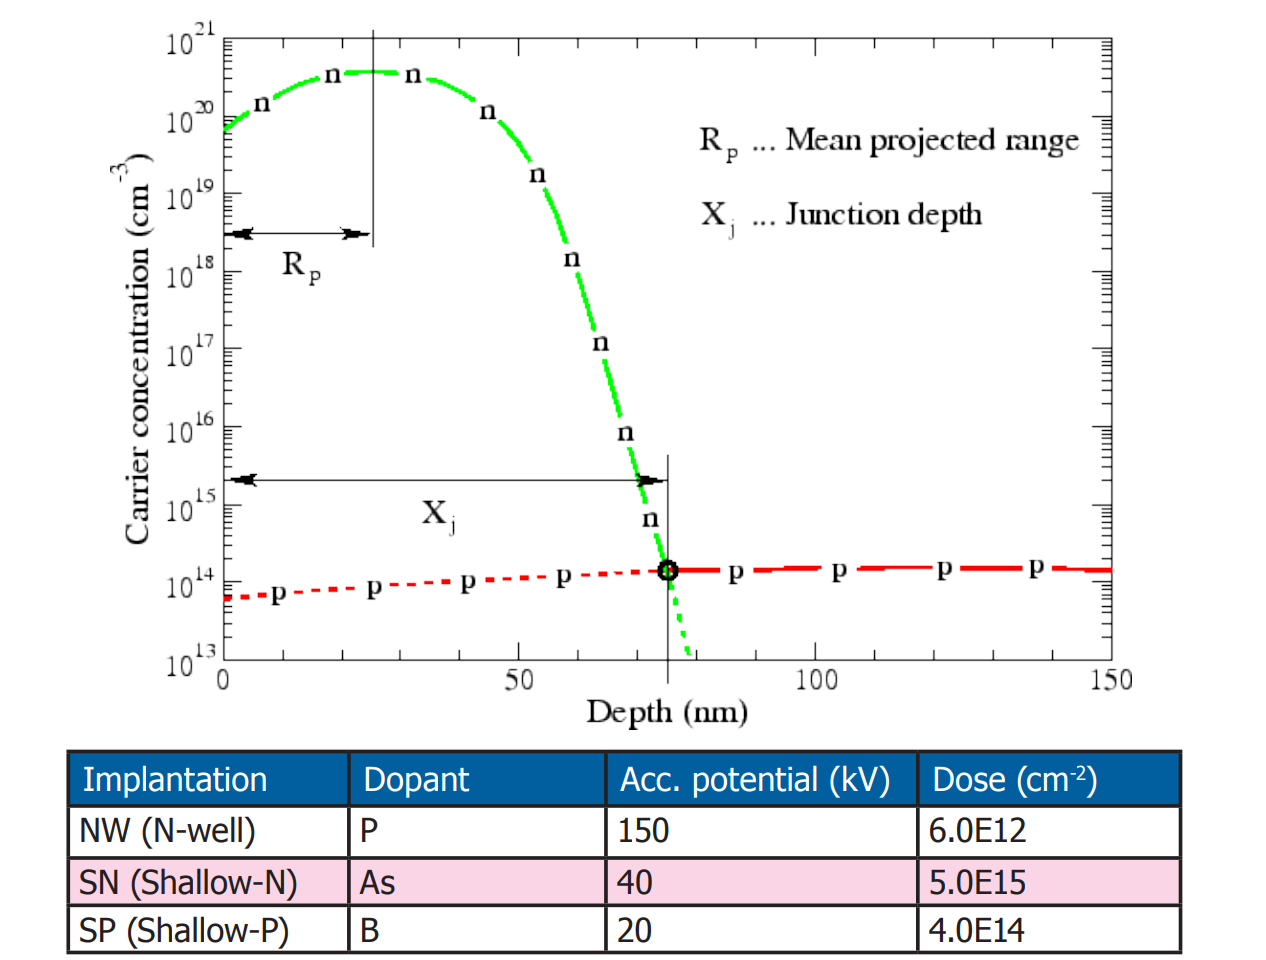
\includegraphics[width=0.7\linewidth]{Figures/tech_assignment_3.png}
    \label{fig:placeholder}
\end{figure}
\noindent \textbf{Knowing the depths of these junctions will be required in order to evaluate the electrical measurements performed in chapters 4 and 6. Here you will calculate the junctions depth, and later compare these with the simulations of chapter 3. All implantations with the used accelerartion voltages are listed in the table above. The goal of this exercise is to perform simple calculations in order to approximate the junction depth.}

\vspace{0.5em}
\noindent \textbf{a) The first implantation is the N-Well. This implantation is also followed by a 4 hours anneal at 1150$^{\circ}$C to drive the P atoms deeper into the surface. If we ignore the implantation depth, we can approximate this process as a limited source diffusion. At 1150$^{\circ}$C the diffusion constant of phosphorus is $8.86 \times 10^{-13} \ \mathrm{cm^2/s}$. Calculate the peak concentration of the implantation and then the junction depth after diffusion, assuming the silicon wafer has a p-type concentration of $10^{16} \ \mathrm{atoms/cm^3}$.}

From the problem statement, if the implantation depth is ignored, the N-Well implantation can be approximated as a limited source diffusion.

For limited source diffusion, the solution to the diffusion equations is then a Gaussian profilet, which is given by
\begin{gather*}
    C(x,t)=\frac{Q}{\sqrt{\pi Dt}}e^{-\frac{x^2}{4Dt}}
\end{gather*}

From the given data, $Q = 6.0 \times 10^{12} \ \mathrm{cm^{-2}}$, $D = 8.86 \times 10^{-13} \ \mathrm{cm^2/s}$ and $t = 4 \ \mathrm{hr} = 14400 \ \mathrm{s}$

The peak concentration occurs at $x=0$, so
\begin{gather*}
    C_{max}=\frac{Q}{\sqrt{\pi Dt}} \\
    C_{max}=\frac{6.0 \times 10^{12}}{\sqrt{\pi(8.86 \times 10^{-13})(14400)}} \approx 2.997 \times 10^{16} \ \mathrm{cm^{-3}}
\end{gather*}

From the problem statement, assume that silicon wafer has a p-type concentration
of $10^{16}$ atoms/cm$^3$, the junction depth is where the phosphorus concentration equals the background p-type concentration:
\begin{gather*}
    C(x,t)=1.0 \times 10^{16} \ \mathrm{cm^{-3}} \\
    1.0 \times 10^{16} = 2.997 \times 10^{16}e^{-\frac{x^2}{4Dt}}
\end{gather*}

Rearrange the equation:
\begin{gather*}
    \frac{1.0 \times 10^{16}}{2.997 \times 10^{16}} = e^{-\frac{x^2}{4Dt}} \\
    \ln \left(\frac{1.0 \times 10^{16}}{2.997 \times 10^{16}}\right) = -\frac{x^2}{4Dt} \\
    x = \sqrt{-4Dt \ln \left(\frac{1.0 \times 10^{16}}{2.997 \times 10^{16}}\right)}
\end{gather*}

Substitute the values:
\begin{gather*}
    x = \sqrt{-4(8.86 \times 10^{-13})(14400)
    \ln \left(\frac{1.0 \times 10^{16}}{2.997 \times 10^{16}}\right)} \approx 2.367 \times 10^{-4} \ \mathrm{cm} = 2.367 \ \mu\mathrm{m}
\end{gather*}

Therefore, the N-Well junction depth is approximately 2.367 $\mu\mathrm{m}$


\vspace{0.5em}
\noindent \textbf{b) The second implantation is the SN and is performed using As in the p-type Si substrate with a concentration of $10^{16}$ boron atoms/cm$^3$. Assuming a Gaussian implantation profile, a projected range ($R_p$) of $0.0314 \ \mu\mathrm{m}$, and straggle ($\Delta R_p$) of $0.0114 \ \mu\mathrm{m}$, calculate the junction depth of the SN implantation using the Gaussian implantation distribution.}

If assume a Gaussian implantation profile, the distribution of the dopant atoms in the silicon is given by the approximation equation below
\begin{gather*}
    N(x)=\frac{Q}{\sqrt{2\pi}\Delta R_p}e^{-\frac{(x-R_p)^2}{2\Delta R_p^2}}
\end{gather*}

From the given data, $Q = 5.0 \times 10^{15} \ \mathrm{cm^{-2}}$, $R_p = 0.0314 \ \mu\mathrm{m}$ and $\Delta R_p = 0.0114 \ \mu\mathrm{m} = 1.14 \times 10^{-6} \ \mathrm{cm}$, the peak concentration is
\begin{gather*}
    N_{max}=\frac{Q}{\sqrt{2\pi}\Delta R_p} \\
    N_{max}=\frac{5.0 \times 10^{15}}{\sqrt{2\pi}(1.14 \times 10^{-6})}  N_{max} \approx 1.75 \times 10^{21} \ \mathrm{cm^{-3}}
\end{gather*}

The junction depth is where the arsenic concentration equals the background boron concentration:
\begin{gather*}
    N(x)=1.0 \times 10^{16} \ \mathrm{cm^{-3}}
\end{gather*}

Therefore,
\begin{gather*}
    1.0 \times 10^{16} = 1.7497 \times 10^{21}e^{-\frac{(x-0.0314)^2}{2(0.0114)^2}} \\
    \frac{1.0 \times 10^{16}}{1.7497 \times 10^{21}} = e^{-\frac{(x-0.0314)^2}{2(0.0114)^2}} \\
    \ln\left(\frac{1.0 \times 10^{16}}{1.7497 \times 10^{21}}\right) = -\frac{(x-0.0314)^2}{2(0.0114)^2} \\
    (x-0.0314)^2 = -2(0.0114)^2
    \ln\left(\frac{1.0 \times 10^{16}}{1.7497 \times 10^{21}}\right) \\
    x^2 - 2(0.0314)x + (0.0314)^2 - 0.0031379 = 0 \\
    x^2 - 0.0628x - 0.0021519 = 0
\end{gather*}

This equation gives two roots, which are $x \approx 0.0874 \ \mu\mathrm{m}$ and $x \approx -0.0246 \ \mu\mathrm{m}$ (discarded). Therefore, the SN junction depth is $0.0874 \ \mu\mathrm{m}$.


\vspace{0.5em}
\noindent \textbf{c) Finally, the SP implantation is done using B. This implantation is performed inside the N-Well, of which you can assume that around the junction the doping concentration is $2 \times 10^{16}$ phosphorus atoms/cm$^3$. Given that $R_p = 0.0685 \ \mu\mathrm{m}$ and $\Delta R_p = 0.0296 \ \mu\mathrm{m}$, calculate the depth of this junction.}

For the SP implantation, the Gaussian implantation profile is again used:
\begin{gather*}
    N(x)=\frac{Q}{\sqrt{2\pi}\Delta R_p}
    e^{-\frac{(x-R_p)^2}{2\Delta R_p^2}}
\end{gather*}

From the given data, $Q = 4.0 \times 10^{14} \ \mathrm{cm^{-2}}$, $R_p = 0.0685 \ \mu\mathrm{m}$ and $\Delta R_p = 0.0296 \ \mu\mathrm{m}$, and convert $\Delta R_p$ from $\mu\mathrm{m}$ to cm:
\begin{gather*}
    \Delta R_p = 0.0296 \times 10^{-4} \ \mathrm{cm}
    = 2.96 \times 10^{-6} \ \mathrm{cm}
\end{gather*}

The peak concentration is
\begin{gather*}
    N_{max}=\frac{Q}{\sqrt{2\pi}\Delta R_p} \\
    N_{max}=\frac{4.0 \times 10^{14}}
    {\sqrt{2\pi}(2.96 \times 10^{-6})} \approx 5.39 \times 10^{19} \ \mathrm{cm^{-3}}
\end{gather*}

The junction depth is where the boron concentration equals the local phosphorus concentration in the N-Well:
\begin{gather*}
    N(x)=2.0 \times 10^{16} \ \mathrm{cm^{-3}}
\end{gather*}

Thus,
\begin{gather*}
    2.0 \times 10^{16}
    =
    5.39 \times 10^{19}
    e^{-\frac{(x-R_p)^2}{2\Delta R_p^2}}
\end{gather*}

Rearrange the equation:
\begin{gather*}
    \frac{2.0 \times 10^{16}}{5.39 \times 10^{19}}
    =
    e^{-\frac{(x-R_p)^2}{2\Delta R_p^2}} \\
    \ln\left(\frac{2.0 \times 10^{16}}{5.39 \times 10^{19}}\right)
    =
    -\frac{(x-R_p)^2}{2\Delta R_p^2} \\
    x = R_p + \sqrt{-2\Delta R_p^2
    \ln\left(\frac{2.0 \times 10^{16}}{5.39 \times 10^{19}}\right)}
\end{gather*}



\vspace{0.5em}
\noindent \textbf{Assignment 4:   BICMOS process flow}

\noindent \textbf{On the next page you see 5 parts of the masks from the BICMOS process. Put the masks in the right processing order and indicate which number corresponds to which process step (e.g. mask 4 is SP mask).}

As mask 4 is SP mask, mask 1 is IC mask, mask 2 is CO mask, mask3 is SN mask, mask 5 is NW mask, the processing order is 5 (NW) $\rightarrow$ 3 (SN) $\rightarrow$ 4 (SP) $\rightarrow$ 2 (CO) $\rightarrow$ 1 (IC)
\begin{figure}[H]
    \centering
    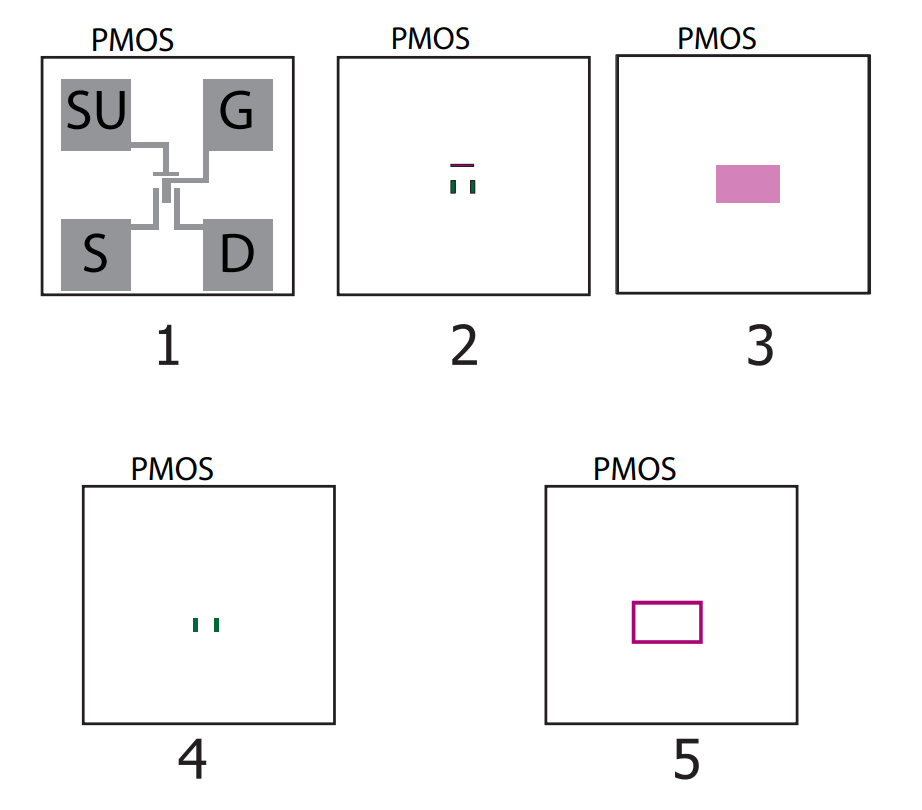
\includegraphics[width=0.5\linewidth]{Figures/tech_assignment_4.png}
    \label{fig:placeholder}
\end{figure}

\vspace{0.5em}
\noindent \textbf{Assignment 5: $V_T$-adjust}

\noindent \textbf{Find the equations which describes the relation between the $V_T$ and the doping levels in the channel for a PMOS and NMOS in literature, and explain why a boron implantation over the whole wafer works as a $V_T$ adjustment for both devices. What happens to threshold voltage of the NMOS when the $VT$-adjust dose is increased? And for the PMOS?}

For NMOS with a channel acceptor concentration of $N_A$, relation between the $V_T$ and the doping levels in the
channel is given by
\begin{equation}
V_{T} = V_{FB} + 2\phi_F + \frac{1}{C_{ox}}\sqrt{2\varepsilon_s\, q\, N_A \cdot 2\phi_F}
\label{eq:vt_nmos}
\end{equation}

For PMOS with a donor concentration of $N_D$, the relation is
\begin{equation}
V_{T} = V_{FB} - 2|\phi_F| - \frac{1}{C_{ox}}\sqrt{2\varepsilon_s\, q\, N_D \cdot 2|\phi_F|}
\label{eq:vt_pmos}
\end{equation}

Boron is a p-type dopant.  The implant adds $N_A$ near the surface of the wafer. Therefore, for NMOS channel, boron adds to the existing acceptor concentration, $N_A$ increases, so $V_T$ becomes larger (NMOS becomes harder to turn on). While for PMOS channel, boron compensates the donors, $N_D$ decreases, so $|V_T|$ decreases ($V_T$ shifts toward zero). Therefore, boron implantation increases magnitude of $V_T$ for NMOS and decreases the magnitude of $V_T$ for PMOS so that NMOS and PMOS device could have threshold voltages which are similar in magnitude.

\newpage